%% The following is a directive for TeXShop to indicate the main file
%%!TEX root = diss.tex

\chapter{Sediment transport and landscape evolution}
\label{ch:Introduction}

\section{Geomorphology traditions}
Geomorphology can be defined as the study of Earth's evolution by tectonics, weathering, and erosion \citep{Chorley1984}. 
This science has long been characterized by observation and description \citep{Gilbert1877, Tight1903, Hack1960}. Only relatively recently did the science turn to quantitative methods \citep{Bagnold1941, Strahler1952, Scheidegger1961, Leopold1962}, with researchers working to frame observations in terms of underlying processes and to describe them with mathematical models modified from physics \citep{Church2005,Roades1996,Chorley1965}.

This quantitative shift or incorporation of physics methods into geomorphology has been criticized as overly reductionist \citep{Slaymaker2020}.
Many of the problems addressed within physics involve closed systems with perfect order \citep{GoldSteinClassicalMechanics,SakuraiQM,JacksonElectrodynamics}. 
These systems stand in contrast to the systems in geomorphology. Earth's surface is open and highly disordered. The surface receives fluxes of mass and energy across its boundaries by tectonics, climate, transpiration, and sunlight, and its component parts vary widely in their characteristics, activities, and compositions. With this complexity \citep{Chorley1971}, we can conclude that a complete reduction of geomorphology to physics is likely impossible.

There are nevertheless lessons physics can exchange with geomorphology and sediment transport theory. This is the central theme of this thesis. Before presenting original research, the first chapter summarizes key developments in quantitative geomorphology models which have resulted from this exchange. The section is organized along two classifications. First, I distinguish earlier works as ``stochastic" or ``deterministic". Stochastic models introduce randomness or noise as a means to crudely represent the complexity of natural systems (open boundaries, diversity in component parts) within idealized mathematical models of nature. Deterministic models involve Newtonian equations without noise to represent nature. Second, I distinguish earlier models as ``discrete" or ``continuous". These terms reflect whether the degrees of freedom of individual particles are retained in mathematical models, or whether they are averaged away. When grains are tracked, a model is discrete. When they are discussed as a flow, it is continuous. We can therefore discuss a ``discrete and stochastic" model, or a ``continuous and deterministic" model, and so on.
With these distinctions in mind, we launch into a survey of the foundation upon which this thesis builds: physics-inspired, process-based models of sediment transport and landscape evolution.

\section{Theories of individual particle movement}

A fundamental problem in sediment transport modelling is to predict the downstream movement of an individual particle.
At first glance, this seems a basic problem in general physics, but digging in exposes severe challenges.
Particles moving as bedload are driven downstream by a turbulent fluid flow \citep{}, but the exact relationships between the fluid flow and the applied forces are not known \citep{Furbish1997}.
Downstream movement is resisted by frictional collisions between moving particles and the bed.
Since the bed is a granular surface, its surface geometry is very difficult to characterize \citep{Gordon1972}, and the outcome of collisions varies from one to the next \citep{Sekine1992}
Entrainment and deposition provide an additional layer of complexity.
Moving particles that encounter the bed with sufficiently low velocities can settle into pockets which protect them from the flow \citep{Miller1966}, so they can deposit \citep{Charru2004}.
These pockets are not permanent shelter.
Rearrangement of the surrounding bed can reexpose sheltered particles to the flow, and sufficiently strong turbulent fluctuations can overcome the shelter, even if the surrounding particles do not move \citep{Valyrakis2012,Celik2014}, so particles can entrain back into motion.
Ultimately, particles at rest on the bed surface can also become covered by other transported particles \citep{Yang1972}. These buried particles cannot move again until those burying them have \citep{Nakagawa1981}.

Predicting the movements of individual particles therefore involves many contributing processes, and our understanding of each of these processes remains incomplete.
\citet{Nikora2001,Nikora2002} provided a conceptual model of individual particle motions which helps to organize this complexity, although it has been slightly revised more recently \citep{Campagnol2013, Hassan2017, Pierce2020}.
Nikora et al divided the downstream trajectory of an individual particle into three timescales, or ``ranges", termed local, intermediate, and global.
The local range refers to the period of motion between subsequent interactions with the bed, when the particle accelerates downstream within the flow, the intermediate range reflects particle motions through sequences of collisions, and the global range refers to particle motion between subsequent entrainment and disentrainment events.
\citet{Hassan2017} added an additional range, referred to as ``geomorphic", to reflect the even longer period over which particles become buried. 
This set of timescales -- local, intermediate, global, and geomorphic -- provides a structure by which to organize wide modelling literature on bedload trajectories and to understand the approximations which have been made on the fundamental problem of predicting the downstream movements of individual grains.


\subsection{Motivation: tracers and basic understanding}
The original motivation to understand individual particle motions was probably to understand the efficiency of sediment transport measurements \citep{Ettema2004}, and this motivation still drives a great deal of research into individual particle motions today \citep{Hassan2017,Pretzlav2021}.
A common measurement technique to estimate sediment transport is to seed a stream with tracer stones and track their progress downstream \citep{Einstein1937, Takayama1966, Ashmore2020}.
In principle, tracers provide a proxy for the population of grains in a stream, so one can estimate tracer velocities of tracers, then multiply by an estimate of the number of grains available for motion in the stream to calculate the overall sediment flux \citep{Yano1969,Nakagawa1976,Hassan2017}.
In practice, challenges arise due to the distinct behavior of tracers over the local, intermediate, global, and geomorphic timescales. Apparently, tracer particle velocities depend on the observation time, in a phenomenon which has been called ``advective slowdown" \citep{Ferguson2002,Haschenberger2012}. This means it is not clear how measured tracer velocities can be mapped back to bulk sediment fluxes, exposing a need for further research into how exactly particle motion characteristics evolve through time.

This need to understand tracer movements is not however the sole point of research into individual particle motions. It is conceptually clear that bulk sediment fluxes ultimately result from the aggregated movements of individual grains, and the prediction of the sediment flux has long been acknowledged as a challenging problem with no clear solution, which impedes geomorphology and engineering understanding \citep{Ancey2020,Ancey2020a}. Better understanding of individual particle motions will support this research.


\subsection{Einstein 1937}
Einstein was probably the first to focus on the movements of individual particles through streams \citep{Einstein1937}, motivated (at least as far as his research supervisor Meyer-Peter was concerned) by the need to understand the efficiency of Helley-Smith samplers for the management of sedimentation \citep{Ettema2004}.
Watching painted tracers move through a flume, Einstein came to the conclusion that the movement characteristics of any one particle could not be predicted, so he turned to probabilistic methods to characterize their transport.
Einstein's key insight was to represent particle motions as an alternating sequence of movements and rests having random characteristics.
As his interest was on the global range of particle motion, and the duration of particle motions is usually short compared to rests, Einstein made the approximation that individual motions (between entrainment and deposition) are mathematically instantaneous.
With this configuration, the downstream movement of sediment becomes an alternate cycle of instantaneous steps of random length, separated by rests of random duration. 
Implicitly, this picture of sediment trajectories assumes that movement velocities are infinite.
Einstein's experiments indicated that both step lengths and resting times were well-described by exponential distributions, and the focus of his PhD was to find the probability density $P(x,t)$ that a particle had travelled a net distance $x$ after a time $t$ has elapsed. He formulated the problem mathematically with an infinite series of convolution integrals, in an elegant display of mathematical physics. 
The mathematics Einstein took on were a pioneering application of the continuous time random walk, which was not formalized until much later \citep{Montroll1965}.


For connection to later work in the thesis, and to provide additional perspective on Einstein's work which is not available in the literature, I will summarize Einstein's work slightly differently than he originally formulated it, using a method based on a stochastic dynamical equation.
In effect, if the position of a single sediment particle at a given time is $x(t)$, the assumptions of infinite movement velocity, random resting durations, and random movement distances between entrainment and depositon (step lengths) can be written
\be \dot{x}(t) = \mu(t), \label{eq:einlangevin}\ee
where $\dot{x} = dx/dt$, and $\mu(t)$ is a white shot noise \citep{VanDenBroeck1983}, which is essentially a sequence of pulses having random heights with mean height $\ell$ (the mean step length), and random locations in time with mean separation $1/k_E$ (the mean resting time, interpreted as the reciprocal of the entrainment rate $k_E$).
A particular realization of this pulsed noise can be written
\be \mu(t) = \sum_{i=1}^{N(t)}s_i \delta(t-t_i), \label{eq:einrando} \ee
where $N(t)$ is the number of particle entrainments in time $t$, distributed as a Poisson distribution $P(N) = e^{-k_E t} (k_E t)^N/N!$, the $t_i$ are distributed according to $P(t) = k_E\exp(-k_E t)$, and the $s_i$ are distributed according to $P(s) = \ell^{-1}\exp(-s \ell^{-1}).$
Figure \ref{fig:einsteinfig} panel (a) sketches this noise, and panel (b) sketches the resulting global range trajectory as a sequence of steps and rests.
Equation \ref{eq:einlangevin} is a kind of dynamical equation representing how the position of a sediment grain evolves through time \citep{Kubo1978}, similar in spirit to Newtonian mechanics \citep{Goldstein1956}, but with a particular random driving term (equation \ref{eq:einrando}) chosen to basically represent the phenomenon under consideration.

\begin{figure}[!htbp]
	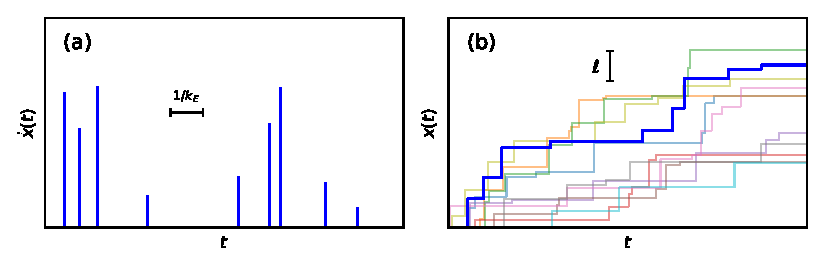
\includegraphics[width=\linewidth,keepaspectratio]{./figures/ch1/einsteinConcept.pdf}
	\caption{Panel (a) indicates the representation of Einstein's model as an idealized ``white shot noise", as indicated in eq. \ref{eq:einrando}, while panel (b) shows the ``stairstep" trajectories of sediment particles moving downstream through cycles of steps (which are instantaneous) and rests (which have mean duration $1/k_E$). }
	\label{fig:einsteinfig}
\end{figure}

The governing equation of the distribution $P(x,t)$ to find the particle at $x$ can be calculated as an ensemble average of $\delta(x-x(t))$ over all possible realizations of the noise \citep{Risken1984,Moss1989}. Different methods exist to compute such averages \citep{Hanggi1978, Hanggi1984, Balakrishnan1993, VanDenBroeck1983}, but whatever the approach, the governing equation for the distribution comes out as
\be  \big(\ell \px \pt + k_E \ell \px + pt \big)P(x,t) = 0. \label{eq:einmaster}\ee
This equation can be solved by standard methods (series solutions or transform calculus) \citep{Arfken1985,Prudnikov1986a} reproduce the original result of \citet{Einstein1937} for the probability distribution of position of a sediment particle:
\be P(x,t) = \delta(x) e^{-k_E t} + e^{-k_E t - x/\ell}\theta(x) \sqrt{\frac{k_E t}{\ell x}}\mathcal{I}_1\Big(2 \sqrt{\frac{k_E x t}{\ell}}\Big) \ee
Here, $\mathcal{I}$ is a modified Bessel function. 
The probability distribution eq. \ref{eq:eindist} fully characterizes the dynamics of an individual particle alternating through steps and rests. 

This distribution displays both advective and diffusive characteristics.
One can calculate all moments of the position by multiplying eq. \ref{eq:einmaster} by $x^n$ and integrating over space. This gives the mean position of the particle
\be \langle x \rangle (t) = k_E \ell t, \ee
so in Einstein's view, sediment grains move with effective velocity $V_\text{eff} = k_E \ell$, given by the entrainment rate times the mean step length.
The rate at which one particle spreads out from another due to differences in their motion characteristics can be represented by the variance of position, $\sigma_x^2  = \langle x^2 \rangle - \langle x \rangle^2$. This gives
\be \sigma_x^2(t) = 2 k_E \ell^2 t, \ee
so particles in Einstein's model spread apart as a normal diffusion process \citep{Sokolev2002}, with an effective diffusivity $D_\text{eff} = k_E \ell^2.$

\subsection{First extensions of the Einstein model}

Einstein's model provides a physically-based model for individual particle trajectories which includes the essential processes at play over global timescales when particles alternate between movement and rest, but it is clearly oversimplified from the reality of particle transport, and a number of extensions and improvements have been made in the 85 years since its development.

Einstein's model of particle movement seems to have been overlooked for the first several decades after its development, or possibly overshadowed by Einstein's later work, which uses its essential ideas for more obviously practical purposes.
Eventually, curiosity into individual particle motions was re-sparked by cold war studies into the fate of radioactive contaminants in river channels \citep{Crickmore1962, Hubbell1964, Sayre1965,Yang1971}, and later by the need to estimate sediment transport rates from tracer measurements \citep{Yano1969, Todorovic1975, Nakagawa1976, Nakagawa1980, Hassan1991}. In relation to these issues, Einstein's model received a great deal of new attention which generated some generalizations of the model.

The first set of modifications to Einstein's approach in this period concerned the form of the distributions used for step lengths and resting times. Einsteins flume experiments demonstrated that particle step lengths followed exponential distributions \citep{1937}, and this was confirmed by subsequent studies \citep{Yano1969, Nakagawa1976}. Yet these studies were all conducted in steady flows in artificial flumes, not real streams, where sediment transport conditions can be different. When sediment transport is observed before and after a flood, rather than during steady flow, the step lengths are better described by a Gamma distribution, this being the sum across the numerous individual steps that occurred during the flood \citep{Hassan1991}. When sediment transport occurs in the presence of dunes or other bedforms, similar modifications have been made to account for spatial differences in transport characteristics \citep{Crickmore1962, Hubbell1964, Sayre1965} and the embedding of particles within bedforms (which increases the periods of rest) \citep{Yang1971,Nakagawa1980}.

\subsection{Inclusion of the movement duration}
\label{sec:lisle}

Einstein's model provides an adequate description of global range particle transport when the period of interest is much larger than the timescales of individual particle movements (local and intermediate ranges) and much smaller than the timescales over which particles embed in the subsurface or other sedimentary deposits (geomorphic range).
Starting in the 1970s, the advent of high speed camera experiments of bed load transporthave produced data on the local and intermediate ranges of particle motion \citep{Abbott1970,Francis1972,Drake1988} which \citet{Einstein1937} never intended to describe.
In the local range, particles move with a fluctuating velocity due to the variable drag of the turbulent flow \citep{Lajeunesse2010,Fathel2015} and changes in the particle's height within the flow profile \citep{VanRijn1984,Wiberg1985}. In the intermediate range, particle-bed collisions impart additional variability to sediment velocities \citep{Gordon1972,Martin2013}.
Einstein's infinite movement velocity assumption excludes the timescales over which these processes occur.

Studies by \citet{Gordon1972}, \citet{Lisle1998}, and \citet{Lajeunesse2017} have generalized the Einstein theory to include the duration of sediment motion. They approximated particle velocities as constant (neglecting fluctuations), and assumed that the movement times are also (along with rests) exponentially distributed random variables, this time characterized by a deposition rate $k_D$, whose reciprocal is the average period of time a particle spends in motion (between entrainment and deposition).
The analogue of Einstein's model equation \ref{eq:einlangevin} with a finite movement velocity $V$ can be written as
\be \dot{x} = V\eta(t), \ee
where the noise is now a so-called ``dichotomous Markov noise" \citep{Bena2006}, which is essentially a random switch or telegraph-type signal that alternates between ``on" ($\eta(t) = 1$) and ``off" ($\eta(t) = 0$) \citep{Cox1965,Horsthemke1984, Masoliver1991, Masoliver1996} as displayed in figure \ref{fig:lislefig} panel (a). Some particle trajectories solving equation \ref{eq:lislelangevin} are displayed in \ref{fig:lislefig} panel (b).

This time, the governing equation of the position probability distribution $P(x,t) = \langle \delta(x-\int_0^t V\eta(t')dt' \rangle$ becomes \citep{Balakrishnan1993}
\be \big(\pt^2 + V \px \pt + k_E V \px + k \pt \big) P(x,t) = 0,\ee
where $k_E$ and $k_D$ are the entrainment and deposition rates, $V$ is the particle velocity during the motion phase, and $k = k_E+k_D$. This partial differential equation is called an asymmetric telegrapher's equation in mathematical physics \citep{Rossetto2018}, and although the symmetric analogue of this equation is well-studied \citep{Weiss2002a, Masoliver2017}, the asymmetric problem is rarely encountered in the literature.

\begin{figure}[!htbp]
	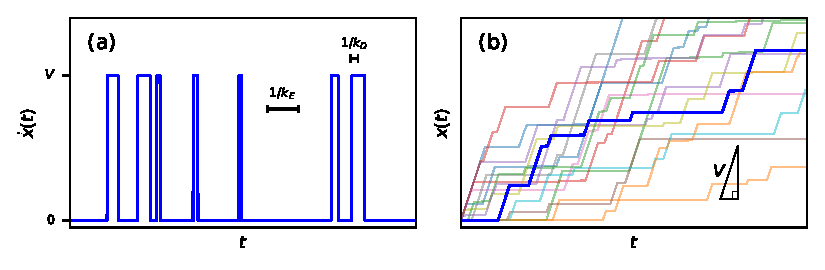
\includegraphics[width=\linewidth,keepaspectratio]{./figures/ch1/lisleConcept.pdf}
	\caption{Panel (a) indicates the generalization of Einstein's model to include the interval of sediment motion between entrainment and deposition, now represented with dichotomous noise eq. \ref{eq:lislerando}, while panel (b) shows the slanted stair-step trajectories of sediment particles moving downstream in cycles of motion at velocity $V$ (with mean duration $1/k_D$) and rest (which have mean duration $1/k_E$). }
	\label{fig:lislefig}
\end{figure}


For the intitial condition that particles have a probability $k_E/k$ to start in motion, the solution of equation \ref{eq:telegraph} is \citep{Lisle1998}
\be \ee
Incorporating the duration of sediment motion, the mean position of the sediment grain remains linear in time: $\langle x \rangle (t) = k_E V t/k$, representing movement at effective velocity $V_\text{eff} = k_E V/k$, which is the fraction of time spent in motion multiplied by the velocity during the motion phase. The variance, however, is different.
Computing $\sigma_x^2$ provides
\be \sigma_x^2(t) = ,\ee
which is a non-trivial result. At short times, for $t\ll 1/k$, equation \ref{eq:lislevar} shows diffusion $\sigma_x^2 \sim t^2$, which is a faster ``ballistic" rate of spreading than the Einstein model predicts \citep{Sokolov2014}. At long times ($t\gg 1/k$), the diffusion becomes normal again ($\sigma_x^2 = 2 D_\text{eff} t$), with an effective diffusion constant $ D_\text{eff} = k_E k_D V^2/k^3$.
In this model, both intermediate and global ranges are adequately represented, but local and geomorphic are not.

\subsection{The Newtonian approach}

Some authors have attempted to model local and intermediate ranges of individual particle trajectories by writing approximate Newtonian equations for the dynamics of individual particles and integrating them numerically. Early efforts impart particles with time-averaged fluid forces, typically linked to a logarithmic flow velocity profile \citep{VanRijn1984}, and some include simplified collision forces that modify particle velocities upon bed contact according to a set of simplified rules \citep{Wiberg1985,Sekine1992}.
Later on, researchers began to include granular interactions among particles to model collisions using the discrete element method \citep{Cundall1979, Haff1993}.
The early works utilizing this approach used a two dimensional domain with a highly simplified flow model \citep{Jiang1993}, while later works have included synthetic turbulence to drive particles \citep{McEwan2001,Schmeeckle2003,Maurin2015} or clever reduced-complexity representations of the flow \citep{Clark2015,Clark2017}.
The state of the art within this category of sediment transport models is to include two-way coupling between particles and the fluid flow. The latter is modelled either by large eddy simulation or direct numerical simulation of the Navier-Stokes equations, using particles as the boundary condition for the fluid \citep{Schmeeckle2014,Ji2013,Gonzalez2017,Vowincklel2014,Elghannay2017,Yousefi2020}.
A next step in this inquiry is to include non-spherical particles, and the foundation for this inquiry is now built \citep{Wachs2011, Azema2012, Wachs2019}.
These computational physics models produce impressive insight into the underlying granular and fluid physics mechanisms producing bed load transport \citep{Frey2011}, but analytically tractable models remain necessary for holistic understanding of sediment transport.

\subsection{Mechanistic-stochastic models for the sediment velocity distribution}

The final set of models relevant to this thesis are the couple of analytical models that have been developed to describe particle velocities in the local and intermediate ranges when velocities fluctuate due to turbulence and particle-bed collisions. These models are indended to apply only between entrainment and deposition.
In contrast to the constant velocities introduced in section \ref{sec:lisle}, the velocities of bed load particles fluctuate through time and are best represented by statistical distributions. 
Among experimental studies on bedload velocities, two dominant conclusions have emerged. One subset of observations indicates that bedload velocities lie on exponential distributions \citep{Lajeunesse2010,Furbish2012,Fathel2015}, and another subset indicates Gaussian distributions \citep{Martin2012,Ancey2014,Heyman2016}.

\citet{Fan2014} set out to describe exponenential-distributed bedload particle velocities with a mechanistic model including a noisy driving term to represent fluid turbulence.
They wrote, for the streamwise particle velocity $u$, a Langevin equation
\be \dot{u}(t) = -\Delta \text{sgn}(u) + F + \sqrt{2D}\xi(t). \label{eq:fanlangevin}\ee
This equation drives the particle velocity by a fluid drag $F + \sqrt{2D} \xi(t)$, where $F$ is a constant, $D$ is a diffusivity that characterizes the magnitude of particle velocity fluctuations, and $\xi(t)$ is a Gaussian white noise with unit variance and vanishing mean \citep{Gardiner1983}. The fluid drag is resisted by a heuristic particle friction term $-\Delta \text{sgn}(u)$, introduced as a proxy for particle-bed collisions. The ``Fokker-Planck equation" governing the probability distribution $P(u,t)$ of the particle velocity can be derived from equation \ref{eq:fanlangevin} as \citep{Risken1984,VanKampen2007} 
\be \pt P(u,t) = \Delta\partial_u\Big[ \text{sgn}(u) P \Big] + D \partial_u^2 P,\ee
implying that the steady-state velocity distribution ($\pt P(x,t) = 0$) provided by equation \ref{eq:fanlangevin} is
\be P(u) = \frac{\Delta^2-F^2}{2\Delta D}\exp\Big(-\frac{-\Delta |u| + F u}{D}\Big).\ee
This is the (two-sided) exponential distribution observed in one subset of the aforementioned experiments.

In a similar approach, \citet{Ancey2014} formulated a Langevin equation to describe the Gaussian velocity distributions observed in the other subset of experiments. They wrote for the streamwise velocity 
\be t_r \dot{u}(t) = -(U-u) + \sqrt{2D}\xi(t),\ee
where $U$ is the mean velocity of particles, $D$ characterizes the magnitude of velocity fluctuations, and $\xi(t)$ is again a Gaussian white noise with vanishing mean and unit variance. The timescale $t_r$ is a relaxation time over which velocity fluctuations decay. This is the well-known Ornstein-Uhlenbeck process of stochastic physics \citep{Gardiner1983}, and its Fokker-Planck equation is
\be \pt P(u,t) = -\partial_u\Big[\frac{U-u}{t_r}P\Big] + \frac{D}{t_r^2} \partial_u^2 P.\ee
This time, the steady state solution becomes
\be P(u) = \sqrt{\frac{t_r}{2\pi D}} \exp\Big(-\frac{t_r(u-U)^2}{2 D}\Big), \ee
which is the Gaussian velocity distribution from the other subset of the experiments.

These models produce successful descriptions of disparate experimental results, although their components are not clearly interpretable in terms of physical expecatations. For example, granular interactions were included in the Fan et al model as a Coulomb friction term. While such approximations are common within Earth science models \citep{Kirkby1971}, they are not entirely satisfying given that bedload particles undergo intermittent collisions with the granular bed. Although these motions are sometimes described as ``sliding", bedload particles do not slide in the same sense as a block on a plane, as the granular term in the Fan et al Langevin model indicates.
In a similar way, the Ancey model does not have a particle-particle interaction term, and it includes what is apparently a Stokes drag term (linear in $u-U$), which is not applicable to bedload transport in water, since bedload particles are typically large compared to the viscous length scale \citep{Clift1978}.
We have to wonder if a more detailed treatment of particle-bed interactions might produce a more general model of bedload particle velocities for application at the local and intermediate scales.

\subsection{Next steps for individual particle motions}


\section{The bulk bedload flux}



\subsection{The definition of the flux}


\subsection{The scaling arguments of Bagnold}

One of the most influential formulations of the bedload flux is due to Bagnold \citep{Bagnold1956,Bagnold1966}, who derived a formula for the mean sediment flux using energy balance arguments.
Bagnold understood sediment transport as a process which converts flow energy to heat via the effective friction \citep{Bagnold1954} of grains against the bed as they move downstream through a succession of collisions \citep{Bagnold1973}.
He assumed that the flow power $P_f$ available to move sediment scales as $P_f \propto \tau - \tau_c$, where $\tau$ is the average bed shear stress and $\tau_c$ is the threshold shear stress at which particles first begin to move. 
Considering that the average downstream flux of particles is $q$, and particles move with mean velocity proportional to the fluid velocity near the bed, Bagnold hypothesized that the power $P_g$ required to sustain particle motion scales as $P_g \propto q/\tau^{1/2}.$
 Balancing flow energy against frictional dissipation ($P_f = P_g$) then provides Bagnold's sediment transport formula
\be q = k(\tau-\tau_c)\tau^{1/2}, \label{eq:bagnold}\ee
which has shown good correspondence with laboratory data at large transport rates, given careful calibration of the constant factors $k$ and $\tau_c$.

The large shear stress limit $q \sim \tau^{3/2}$ of Bagnold's formula is shared in common with many other empirical formulas describing the mean downstream flux of bedload \citep[e.g.][]{MeyerPeter1948, Yalin1972, Wilcock2003, Parker1998}. The distinguishing feature of Bagnold's formula is its derivation from mechanical principles, although many of the details have turned out to be incorrect. For example, Bagnold's assumption that the power available to move sediment scaled with the excess shear stress leads to unphysical results over arbitrarily sloping beds \citep{Seminara2002}, and in reality, the flow power dissipated by sediment transport shows only a weak correlation the sediment flux \citep{Ancey2008}, while Bagnold assumed they were directly proportional. These issues have been hinted when calibrating Bagnold's formula to data, where the parameters $k$, which is related in Bagnold's formalism to the angle of repose of sediment, and $\tau_c$ take on unphysical values at low transport rates \citep{Nino1996}.
Finally, Bagnold's formulation faces the notorious challenge of defining the critical shear stress $\tau_c$ for the initiation of sediment transport \citep{Paintal1971,Kirchener1990,Houssais2015,Clark2017,Allen2018}, which is a topic for another thesis. 
The difficulties with Bagnold's approach led many followers to revise his theory, merging his approach, which is based on Bagnold's characteristically sharp physical insight, with new experimental conclusions on the energetics of sediment transport \citep{Engelund1976,Luque1976,Nino1998,Martin2000}.

\subsection{Einstein's probabilistic approach}

Among these revisions of Bagnold, one category shows a return to the probabilistic ideas of Einstein \citep{Parker2003,Ancey2006}.
Einstein's formulated his original model of individual grains in transport \citep{Einstein1937} in terms of particle entrainment and deposition, supplemented with the idea that grains move downstream through a sequence of instantaneous steps.
Later, \citet{Einstein1942,Einstein1950} formulated the bulk sediment flux using these same ideas, providing an alternative to Bagnold based on probabilistic arguments.
The conceptual picture that Einstein considered is depicted in figure \ref{fig:einsteinFluxConcept}.
 \begin{figure}[!htbp]
	\includegraphics[width=\linewidth,keepaspectratio]{./figures/ch1/yalinDrawing.pdf}
	\caption{Einstein’s conceptual picture (modified from \citet{Yalin1972}). Particles move in discrete jumps of length $\ell$ from
left to right through an array of adjacent control volumes. The bedload flux is the volume (or number) of bedload particles crossing
the surface $\mathcal{S}$ per unit width and time.}
	\label{fig:lislefig}
\end{figure}

To derive the mean bedload flux, Einstein partitioned the channel into a sequence of identical control volumes $V$, and calculated the average rate at which particles cross a control surface by aggregating the contributions from each upstream control volume.
Each control volume has downstream length $\ell$ which is also the average particle step length.
Denoting by $P_n$ the probability that an individual grain undergoes at least $n$ jumps of length $\ell$ in a time interval $T$, meaning it travels at least a distance $n \ell$, and that there is a density $\rho$ of particles at rest on the bed, it follows that on average $\rho \ell P_n$ particles will displace a distance $n \ell$ or more from each control volume within the time interval $T$. 
As a result, since grains crossing $\mathcal{S}$ in a time $T$ could have come from any upstream location, the number of grains crossing $\mathcal{S}$ in $T$ is a sum over all control volumes: $\sum_{n=1}^\infty \rho \ell P_n$.
Dividing by the time $T$ to get the average rate of grains crossing $\mathcal{S}$ gives the mean flux
\be q = \frac{\rho \ell}{T} \sum_{n=1}^\infty P_n. \label{eq:einflux} \ee
The reamining quantity to evaluate is $P_n$, the probability a particle entrains \textit{at least} $n$ times in a time $T$.

Einstein originally constructed this probability by assuming that each particle had $n$ independent entrainment opportunities in the period $T$, each with probability $p$, so that $P_n = p^n$, but this approach has been critiqued by \citet{Yalin1972} and others \citep{Paintal1971,Cheng2004,Armanini2015,Armanini2017}. Instead, one should calculate $P_n$ as an exceedance probability.
If the entrainment rate of an individual grain is $k_E$ (probability per unit time), then the probability that it entrains \textit{exactly} $n$ times in time $T$, denoted by $p_n$ (distinct from $P_n$!) is a Poisson distribution:
\be p_n = \frac{(k_E T)^n}{n!}e^{-k_E T}.\ee
This implies that the probability that it entrains \textit{at least} $n$ times is $P_n = \sum_{i=n}^\infty  \frac{(k_E T)^n}{n!}e^{-k_E T}, $
so Einstein's mean sediment flux (eq. \ref(eq:einflux}) becomes
\be q = \frac{\rho \ell}{T} \sum_{n=1}^\infty \sum_{l=n}^\infty = \frac{\rho \ell}{T}\sum_{n=1}^\infty n \frac{(k_E T)^n}{n!}e^{-k_E T} = \rho k_E \ell.\ee
Noticing that $\rho k_E$ is the entrainment rate of a single grain multiplied by the density of grains available for entrainment on the bed, we can write 
\be q = E \ell \ee
as the central result of Einstein's theory. Here, the quantity $E = \rho k_E$ is the areal entrainment rate, representing the number of grains entrained per unit bed area \citep{Wilcock1997,Furbish2012}.

Alongside the central result $q=E\ell$ for the mean flux, one of Einstein's most influential and enduring ideas was his formulation of the entrainment rate $k_E$ of the individual particle in terms of the force balance on the stationary particle.
The original approach considers that entrainment is driven by the fluctuating lift force imparted by the turbulent flow, and it is resisted by the submerged weight the grain.
The entrainment rate is calculated from the exceedance probability of the turbulent lift over the weight, providing an alternative to the critical shear stress concept which explicitly incorporates turbulent fluctuations in the fluid flow. This formulation of entrainment probability in terms of the exceedance of random driving quantities over (possibly
random) resisting quantities \citep{Grass1970} is a key part of Einstein's legacy. \citet{Paintal1971} made a significant extension
by including the random supporting geometry of bed particles into the force balance. More recently, \citet{Tregnaghi2012}
ammended the theory to include both force magnitude and duration \citep{Diplas2008, Valyrakis2012, Celik2014}.
Refined theories of the single-particle entrainment rate, all fundamentally similar to the original ideas of \citet{Einstein1950}, have been carefully reviewed by \citet{Dey2018} and remain under active development.

\subsection{Fusing Einstein and Bagnold}

Although Einstein worked to relate $k_E$ to the flow, other parameters of Einstein's model ($\rho$, $\ell$) retain a heuristic character which is not clearly linked to the underlying fluid-granular physics. The erosion-deposition model originally developed by \citet{Charru2004,Charru2006,Charru2006a} relates the central parameters of the Einstein model to properties of the flow using scaling relations \citep{Charru2004, Charru2006, Lajeunesse2010,Seizilles2014,Lajeunesse2015}.
This can be characterized as a mixture of the Einstein and Bagnold strategies.

Derived by evaluating mass balance within a control volume, the erosion-deposition model is
\be \pt \gamma +  \px V \gamma = E - D. \label{eq:charru}\ee
In this equation, $\gamma$ is the ``particle activity", which is the number of moving particles per unit area \citep{Furbish2012}, $V$ is the ensemble average movement velocity of sediment grains (which in unsteady conditions may depend on space and time), $E$ is the entrainment rate (the number of particles transitioning to motion per unit area and time), and $D$ is the deposition rate (the number of particles coming to rest on the bed per unit area and time).

Scaling arguments provide relations for $E$, $D$, and $V$ in terms of the fluid shear stress $\tau$, particle size $d$, particle settling velocity $V_s$, and the critical shear stress $\tau_c$:
\be E = a \frac{\tau-\tau_c}{d^3 V_s}, \label{eq:charru1}\ee
\be D  = b\frac{\gamma V_s}{d}, \ee
\be V = c + d(\sqrt{\tau}-\sqrt{\tau_c}). \label{eq:charru2}\ee
The constant coefficients $a$, $b$, $c$, and $d$ are determined experimentally.

Equation \ref{eq:charru} indicates that the mean flux in steady transport conditions is the implicit solution to the equation $E = D.$
Using the scaling relations \ref{eq:charru1} and \ref{eq:charru2} provides the mean particle activity
\be \gamma \propto \frac{\tau-\tau_c}{d^2 V_s^2}.\ee
Expressing the mean flux as $q = \gamma V$, in the control volume interpretation, the relationship between flux and bed shear stress becomes
\be q = \frac{A}{d^2 V_s^2}\big(\tau-\tau_c\big)\big[c + d(\sqrt{\tau}-\sqrt{\tau_c})\big]. \ee
This recovers the Bagnold scaling $q \propto \tau^{3/2}$ at large bed shear stresses.

\subsection{The nonlocal formulation}

Einstein's model of the bulk bedload flux is inherently nonlocal in that it aggregates particle motions from all upstream locations \citep{Schumer2009}.
\citet{Parker2000} formalized this by writing the sediment flux in an explicitly nonlocal form:
\be q(x,t) = \int_0^\infty dx' F(x-x',t)E(x',t). \ee
In this equation, motions are instantaneous, and $F(x,t)$ is the probability that a just-entrained particle steps a distance $l$ before deposition.

\citet{Furbish2012} generalized the Parker model to include a finite duration of motion.
They wrote
\be q(x,t) = \int_0^\infty dx' \int_0^\infty dt' F(x',t') E(x-x',t-t'), \label{eq:furbo}\ee
where, $F(x,t)$ represents the probability density that particles move \textit{at least} a distance x in time $t$ (right after entrainment).
For a simple example of the Furbish et al formalism, consider particles that move with a constant velocity $V$ and have a deposition rate $k_D$. 
Then the probability density that a particle moves \textit{exactly} a distance $x$ in time $t$ is $f(x,t) = \delta(x-Vt)k_D\exp(-k_D t), $ so the probability that it moves 
\textit{at least} a distance $x$ in $t$ is
\be F(x,t) = \int_0^t \delta(x-Vt)k_D\exp(-k_D t) = \theta(Vt-x)k_D\exp(-k_D t).\ee
Considering uniform conditions with a density $\rho$ of particles available for motion on the bed surface, each having entrainment rate $k_E$, the bulk entrainment rate can be expressed as $E=\rho k_E$, and equation \ref{eq:furbo} provides a mean flux
\be q = \rho k_E \int_0^\infty dx' \int_0^\infty dt' \theta(Vt-x)k_D\exp(-k_D t) = \rho k_E V/k_D. \label{eq:furbflux}\ee
Since $1/k_D$ is the average time spent in motion, $V/k_D$ is the average step length $\ell$. Equation \ref{eq:furbflux} provides another perspective on Einstein's result $q= E\ell$.

Furbish et al also provided a local approximation of the nonlocal flux expressed equation \ref{eq:furbo}. This result is useful for unsteady conditions when spatial gradients occur in the particle activity.



\subsection{The connection to landscape evolution}

Exner was probably the first to write the mathematical relationship between sediment transport and topographic change \citep{Exner1925}. He wrote
\be (1-\lambda)\frac{\partial z}{\partial t}(\textbf{x},t) = -\nabla q (\textbf{x},t). \ee
This equation links the temporal evolution of the land elevation $z$ at a location $\textbf{x}=(x,y)$ to spatial gradients in the sediment flux $q$. The parameter $\lambda$ is the bed porosity.

Within the Exner equation, the elevation $z$ and sediment flux $q$ are represented as continuous fields. This representation can be interpreted as an average over the detailed locations of individual grains, and it is expected valid whenever the scales of interest are large compared to the size of the averaging window, which should be taken much larger than the size of the largest grains being modelled \citep{Coleman2009}. 
Yet there are many contexts on Earth's surface where the scale of interest is not much larger than the largest grains involved in the system. We can wonder, for example, in mountain channels, how large boulders control to the formation of steps \citep{Church2007,Zimmerman2008,Saletti2020}, or other structures with sizes comparable to channel widths, like ribs or stone cells \citep{Hassan2008,Venditti2017}. In these cases, individual grains are comparable to the scales of interest, and the continuum description provided by the Exner equation seems questionable.



\subsection{Fluctuations and scale dependence}

\subsection{Birth death models}

\subsection{Queueing theories}

\subsection{Next steps for the bedload flux}


\endinput



\section{Bedload transport foundations}

In river science, a fundamental problem is the determination of the bedload flux, or the rate of downstream movement of coarse sediment grains \citep{Ballio2014}.
Since bedload transport has strong feedback with stream morphology \citep{Church2006, Recking2016}, its prediction is useful to a wide range of environmental considerations. 
These considerations span a wide range, from aquatic habitat restoration to energy production \citep{Kondolf2014, Wohl2015a}. 
Unfortunately, no satisfying approach currently exists to compute the bedload flux \citep{Ancey2020,Ancey2020a}, and predictions regularly deviate by two orders of magnitude from measured values \citep{Gomez1989, Barry2004, Bathurst2007a, Recking2012}. 

Predicting bedload fluxes is challenging because transport is not always well correlated to average characterizations of flow and bed material. 
Local fluxes can range through orders of magnitude as details of turbulent fluctuations and bed organization vary, while average characterizations of flow and sediment remain constant \citep{Sumer2003, Charru2004, Hassan2008, Venditti2017}.
The same turbulence and bed sediment organization details which correlate with the bedload flux are also modified by it.
Turbulent impulses induce sediment motion \citep{Valyrakis2010, Celik2014, Amir2014, Shih2017}, while moving sediment affects turublence characteristics \citep{Singh2010, Santos2014, Liu2016}, and bedload transport modifies the stability and arrangement of bed surface grains \citep{Kirchener1990, Charru2004, Hassan2008}.
The bedload flux is in a cyclical feedback with its control variables, the details of turbulence and bed organization \citep{Jerolmack2005}. 

\subsection{Bulk bedload flux}

Perhaps a surprising outcome of over a century of bedload transport research is that no one definition of the sediment flux has yet been agreed upon.
Today, there are two main competing (or complementary) approaches to define the bedload flux. 
The first definition is reminiscent of continuum mechanics or electrodynamics \citep{Landau, Jackson19xx}, and formulates the flux as a kind of current of sediment across (normal to) a control surface $\matchal{S}$ \citep{Furbish2012,Heyman2016}: 
\be q = \int_\mathcal{S} c(\textbf{x},t)\textbf{u}\cdot d\textbf{\mathcal{S}}. \ee
This definition involves the concentration $c$ of particles in space and their velocites at the instant they cross the control surface, which is a somewhat elusive quantity since bedload particles are not a continuous field over the scales of interest \citep{Heyman2016}.
Lately, this concentration has been interpreted as an ensemble average \citep{Furbish2012,Ballio2014}.
The second definition formulates the downstream flux in terms of the number of particles moving within a control volume $\mathcal{V}$:
\be q = \frac{1}{L} \sum_{i\in\mathcal{V}} u_i.\ee
Here, the flux is evaluated as a sum over all downstream velocities of particles within the volume (of which there are a fluctuating number), and the division by the downstream length of the control volume is incorporated to count only that proportion of particles near the downstream boundary of the volume.

\subsection{Bagnold's energy balance}





\subsection{Discrete particle models}


\subsection{The probabilistic approach of Einstein}


\section{From transport to landscape evolution}


\subsection{Exner's approach} 

 


\subsection{Tusjimoto and beyond}
Explain what tsujimoto essentially did to couple Einstein into Exner, giving the entrainment form of the exner equation.
Cite Parker and Furbish who provided refinements of it.
Describe the inherently nonlocal characteristics of sediment flux.
Indicate the major strengths and weaknesses -  key weakness being that, if the sediment flux is a fluctuating quantity, as formulated by Einstein, then 

\section{Topics and organization of the thesis} 




\subsection{Organization of the thesis}

Four main problems. Ch 2 is about how to calculate the sediment flux and to understnad particle motion with fluctuating velocities.
Ch3 is a sketch of how we can incorporate bed elevation changes into sediment transport modelling based on stochastic theories.
Ch4 is the 

\section{Introduction: birth-death models for the probability distribution of bedload flux}

In river science, a fundamental problem is the determination of the bedload flux, or the rate of downstream movement of bedload grains \citep{Ballio2014}.
Since bedload transport has strong feedback with stream morphology \citep{Church2006, Recking2016}, its prediction is useful to a wide range of environmental considerations. 
These considerations span a wide range, from aquatic habitat restoration to energy production \citep{Kondolf2014, Wohl2015a}. 
Unfortunately, existing approaches to compute the bedload flux are inadequate. 
Predictions regularly deviate by two orders of magnitude from measured values \citep{Gomez1989, Barry2004, Bathurst2007a, Recking2012}. 

Predicting bedload fluxes is challenging because transport is not always well correlated to average characterizations of flow and bed material. 
Local fluxes can range through orders of magnitude as details of turbulent fluctuations and bed organization vary, while average characterizations of flow and sediment remain constant \citep{Sumer2003, Charru2004, Hassan2008, Venditti2017}.
The same turbulence and sediment organization details which correlate with the bedload flux also interact with it. 
Turbulent impulses induce sediment motion \citep{Valyrakis2010, Celik2014, Amir2014, Shih2017}, moving sediment affects turublence characteristics \citep{Singh2010, Santos2014, Liu2016}, and bedload fluxes modify the stability and arrangement of bed surface grains \citep{Kirchener1990, Charru2004, Hassan2008}.
The bedload flux is in a cyclical feedback with its controls: these controls are the details of turbulence and bed organization \citep{Jerolmack2005}. 

As a result, bedload fluxes exhibit wide fluctuations, even as average characterizations of flow and bed organization remain steady \citep{Ancey2014}.
In the most controlled laboratory experiments, with steady flows driving uniform glass beads under conditions which do not favor bedform development, instantaneous fluxes are often as much as 200\% mean values \citep{Bohm2004, Ancey2008, Heyman2014, Heyman2016}. 
In natural streams, with temporally or spatially varying grain size distributions \citep{Lisle1992, Chen2008}, unsteady flows \citep{Mao2012, FerrerBoix2015}, a variety of dynamic bed surface structures \citep{Hassan2008, Venditti2017}, variable sediment supply \citep{Madej2009, Elgueta2018}, lateral adjustment \citep{Pitlick2013, Redolfi2018}, and migrating bedforms \citep{Gomez1989, Dhont2018} all imparting additional sources of variabilility through their feedbacks with the flux, instantaneous fluxes can be even larger. 
% Iseya1987, Lisle1989, Kuhnle1998

Apparently, bedload fluxes have statistical characteristics.
Einstein was the first to recognize the statistical character of bedload transport \citep{Einstein1937}. 
He understood transport as a random switching between states of motion and rest \citep{Einstein1942, Einstein1950}. 
He called the transition from rest to motion entrainment, and he characterized it with a probability which was linked to extreme events in fluid turbulence \citep{Einstein1949, Einstein1950}. 
He called the transition from motion to rest deposition, and he considered it an implicit function of the bedload flux \citep{Einstein1942, Einstein1950}. 
By convolving over sequences of entrainment and deposition, employing some semi-emprical arguments, Einstein developed a formula for the average bedload flux \citep{Einstein1950}. 

Many investigators have criticized and developed Einstein's ideas \citep{Paintal1971, Yalin1972, Shen1980, Lisle1998, Papanicolaou2002, Sun2000, Ancey2006, Armanini2015}. 
These revisions focus on the more simplified aspects of Einstein's derivations, and they lend a more mechanistic basis, a firmer mathematical foundation, and more generality to the approach. 
Although all of these authors accepted the statistical character of bedload motion, none developed theories for a probability distribution for the bedload flux. 
This is desirable since its higher moments give unambiguous measurements of the magnitude of bedload fluctuations. 

The extension of the Einstein approach to obtain a probability distribution of the bedload flux, with fluctuations stemming from the random character of entrainment and deposition, was first explored by \citet{Lisle1998, Sun2000}, and it was further developed by \citet{Ancey2006}, and the more recent work I will discuss extensively in this review.   
All of these authors revisited Einstein's ideas from a foundation in the stochastic mathematics which became formalized somewhat after Einstein's work \citep[e.g.][]{Cox1965}, treating the transitions between motion and rest states as random events characterized by probabilities. 
This enabled them to apply the formalism of continuous time Markov processes to derive a probability distribution of the bedload flux, with a mean value which was an improved version of the \citet{Einstein1950} formula, very similar to the revised formula of \citet{Yalin1972}, and a variance which provided an unambiguous prediction of the magnitude of bedload fluctuations. 

Deterministic processes trace the evolution of some set of variables $\{x_1(t),x_2(t),\dots\}$ through time. 
Stochastic processes, in contrast, trace the evolution of a probability distribution for random variables $P_{X_1,X_2,\dots}(x_1,x_2,\dots;t)$ through time. 
The Markov moniker refers to the amount of memory in the process.
If the probability distribution of the variables of interest can be predicted in the future using only distribution functions from the present, the process is Markovian. 
Otherwise, if predicting the future requires knowledge of the entire history, the process is non-Markovian \citep{Cox1965, VanKampen1992}. 
Markov birth-death processes consider the probabilistic creation and annhilation of members of a population \citep{Cox1965, VanKampen1992}.  

To model the bedload flux with such a process, the population considered is the number of moving particles within a control volume over the bed. 
This population is subject to creation by entrainment and annhilation by deposition \citep{Ancey2008, Turowski2009, Heyman2013, Ma2014,  Ancey2014a, Ancey2015}. 
This approach is exciting because Markov birth-death processes are highly studied in physics, chemistry, and population ecology, so there are many extensions readily available \citep{Bailey1968, Cox1965, Pielou1977, VandenBroek2012, VanKampen1992, Gillespie1992, Field2010, Mendez2015}. 
At the same time, birth-death modeling of the bedload flux remains relatively undeveloped: birth-death models are all one-dimensional and designed for a single grain size. 

In this article, I review the literature on Markov birth-death models of the bedload flux.
In the review I assume some familiarity with discrete state continuous time Markov processes, which could be gleaned from reading the appropriate chapter in \citet{Cox1965}. 
These theories are exciting because they describe the mean bedload flux and its fluctuations within a volume \citep{Ancey2006, Ancey2008, Turowski2009}, statistical properties of the flux at a point in space \citep{Heyman2013, Ma2014}, and the spatial and temporal correlations in the bedload flux within a reach of channel \citep{Ancey2014, Ancey2015}. 
All of these considerations are new, and they are unique within the river science literature in that they do not ignore the statistical character of bedload transport. 
They initiate a theoretical framework from which the feedbacks between the arrangement of bed particles, turbulence, and channel morphology which lead to bedload fluctuations can be more carefully studied and understood. 
In reverse, the capacity of bedload models to describe fluctuations provides an additional benchmark against which to judge models, a task which is notably difficult \citep{Iverson2013}. 

One of the first birth-death models of the bedload flux I will review is \citet{Ancey2006}: these authors generalized \citet{Einstein1950} using a birth-death framework to obtain a statistical distribution of the bedload flux within a control volume. 
They found the fluctuations predicted by the Einstein-like model were not large enough to describe experimental data.  
In order to match the wide fluctuations of experimental data, \citet{Ancey2008} reworked their earlier control volume model to include a collective entrainment effect.
Collective entrainment is a mathematical term charaterizing the correlations between moving grains due to turbulence, collisions, or granular avalanche effects.

The \citet{Ancey2008} model has been generalized and applied in a handful of followup works. 
\citet{Turowski2009} generalized it to include limited sediment availability. 
\citet{Heyman2013} and \citet{Ma2014} studied how the \citet{Ancey2008} model could be interpreted to describe the statistics of the bedload flux at a fixed point in space, rather than just a control volume like that considered by \citet{Einstein1950}. 
Control volumes are less desirable because transport is practically easier to measure at a point in space than it is within a control volume. 

\citet{Ancey2014, Ancey2015} generalized the \citet{Ancey2008} model in order to understand spatial characteristics of bedload transport. 
They considered a reach of channel as an array of adjacent control volumes (cells), and they coupled the \citet{Ancey2008} model between adjacent cells. 
They mapped this generalized birth-death model for the bedload flux distributed over an array of control volumes onto an advection diffusion equation for the bedload flux. 
Some reprecussions of this model were further explored in context of experimental data by \citet{Heyman2014}. 

All of these works contain many simplifying assumptions, and many of these were carefully highlighted by their authors. 
These studies were selected for this review because, taken together, they define a research trajectory which can be extrapolated to suggest future research topics. 
To be sure, there is a long road ahead before Markov models can accomodate all of the complexities of natural river channels, some of which I've mentioned. 
The goal of this review is to indicate this trajectory in order to motivate future research: this is pursued in sections \ref{sec:background} and \ref{sec:review}. 
I discuss some of the future research topics I believe the trajectory points out in section \ref{sec:scope}, and I develop a few of these ideas myself in \ref{sec:extension}. 
Along the way, I have somewhat changed the mathematical treatment and the notation from some of the original papers in order to highlight the historical progression between each work, and to illustrate that these works all share the same theme.  




\section{Background: the foundational stochastic model of bedload transport} 
\label{sec:background}

\citet{Einstein1950} can be credited with the first attempt to understand the bedload flux as random quantity.  
Einstein understood the movement of individual bedload grains as a random succession of motion and rest intervals.
He termed the transition from rest to motion entrainment, and characterized it by a probability related to fluid turbulence. 
When particles are set in motion, Einstein considered they moved in discrete jumps of the same average distance. 
We define the bedload flux as the volume of grains passing a stream cross section per unit time.
It is a volume of grains per time per unit width of stream, so its units are $\text{area}/\text{time}$.  
Therefore, Einstein's mean flux formula is derived from summing the alternate start-stop motions of all bed particles which cross a surface in a time interval. 

The conceptual picture Einstein considered is depicted in figure \ref{fig:yalin}. 
All bed particles are identical and are considered to have the same average geometry when at rest on the bed, meaning their entrainment characteristics are identical. 
For continuity with the rest of the review, we consider sediment particles are spheres of radius $a$, although \citet{Einstein1950} was more general. 
We can follow Einstein to compute the mean number of these particles crossing a flow cross-sectional surface $S$ in an interval of time. 
This will construct the mean bedload flux $\bra q_s \ket$.
In subsequent sections, we consider $q_s$ a random variable, and we will review approaches to derive its full probability distribution.
From these contemporary models, an Einstein-like mean flux formula emerges from taking the mean of the probability distribution for $q_s$.  
Hence we use averaging brackets $\bra \cdot \ket$ for the sake of continuity. 

\begin{figure}
	\centering
	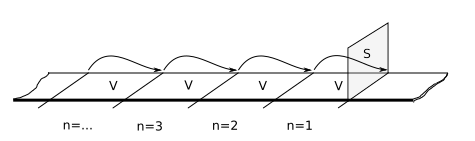
\includegraphics[width=.98\linewidth]{./figures/ch1/yalindrawing.png}
	\caption{Einstein's conceptual picture (adapted from \citet{Yalin1972}). Particles move in discrete jumps of length $L$ from left to right through an array of adjacent control volumes. The bedload flux is the volume of bedload particles crossing the surface $S$ per unit width and time. \label{fig:yalin}}
\end{figure}

Einstein's derivation goes as follows: we partition the channel into a sequence of identical control volumes $V$. 
Each volume has dimensions $L$, $w$, and $h$ ($V=lwh$). 
$L$ is the downstream length of each control volume, and it is also the average jump distance of particles. 
$w$ and $h$ are the width and height of each control volume.
Let $P_n$ be the probability that any individual grain on the bed is entrained \textit{at least} $n$ times during the time interval $T$. 
That is, let $P_n$ be the probability that an individual grain undergoes \textit{at least} $n$ jumps of length $L$ in an interval $T$, meaning it travels a distance $nL$ or more in $T$. 
Considering that each control volume contains $N_V$ grains at rest within it, it follows that on average
\be N_V P_n. \ee
grains are displaced \textit{at least} a distance $nL$ from a control volume within the time interval $T$.

Now we derive the mean flux. 
Note that the grains passing through a cross-sectional surface $S$ (of area $lw$) in the time $T$ could have come from any upstream location. 
Therefore, the number of grains crossing $S$ in $T$ is 
\be \sum_{n=1}^\infty N_V P_n. \ee
This is the net arrival of grains in the interval $T$ from all upstream control volumes. 
Multiplying by the particle volume $\nu_p$ and dividing by the timescale $T$ and channel width $w$ gives the mean bedload flux (volume per width per time):
\be \bra q_s \ket = \frac{\nu_p N_V}{w T}\sum_{n=1}^\infty P_n = A \frac{a^2}{T} \sum_{n=1}^\infty P_n. \label{eq:einstein1}\ee 
In the second equality, we have introduced $\nu_p = 4\pi a^3/3$, and two assumptions of Einstein. First, is the reasonable assumption that the number $N_V$ of particles on the surface within $V$ is proportional to the ratio of bed surface and particle areas: $N_V \propto Lw/a^2$, and second is the assumption that the travel distance $L$ is proportional to particle size: $L \propto a$. The latter assumption is more difficult to justify \citep[e.g.][]{Yalin1972}. 
$A$ is a constant of proportionality. 

Einstein implies the probability that an individual grain travels a distance $nL$ or more in $T$ is equivalent to the probability that an individual grain travels at least a distance $L$ successively $n$ times in $T$. 
Hence $P_n = P_1^n$ by the law of multiplication of probabilities, so that $\sum_{n=1}^\infty P_n = \sum_{n=1}^\infty P_1^n = P_1/(1-P_1)$, using the geometric series (noting $P_1 < 1$ because it is a probability). 
Owing to this substitution, Einstein's mean bedload formula takes the form 
\be  \bra q_s \ket = A \frac{a^2}{T}\frac{P_1}{1-P_1}, \label{eq:einstein2} \ee
where $A$ is a constant of proprotionality.  
The $P_1/(1-P_1)$ structure of Einstein's formula is a distinctive characteristic. 
In order to use the apply the Einstein formula to predict bedload transport in natural streams or experiments, the timescale $T$ and the probability $P_1$ that at least one grain entrains in $T$ must be determined. 
Then the formula can be calibrated to a given setting by adjusting the constant $A$.  

In the original work, Einstein considered the timescale $T$ proportional to the "time of the grain" formed by the grain's size $a$ and its settling velocity $w$ in still fluid: $T \propto a/w$. 
We will revisit this assumption shortly. 
Regarding the probability $P_1$, one of Einstein's most influential and enduring ideas within hydraulic engineering is his conception of the probability $P_1$ that at least one particle entrains in $T$. 
He considered that entrainment is driven by the fluctuating lift force imparted by the turbulent fluid, and it is resisted by the submerged weight of grains. 
Therefore, he formulated $P_1$ as an exceedance probability of the lift force over weight, so he wrote $P_1$ as an integral over the probability distribution of fluid shear stress. 
Einstein developed an alternative perspective on the incipient motion of particles that embraced turbulence and did not rely on the critical shear stress concept \citep[e.g.][]{Shields1936}.

This formulation of entrainment probability in terms of the exceedance of random driving quantities over (possibly random) resisting quantities has been generalized and extended a great deal. 
\citet{Paintal1971} made a significant extension by including random granular geometry of bed particles into the force balance. 
More recently, \citet{Tregnaghi2012} ammended the theory to include the impulse concept: the experimentally verified idea that force magnitude and duration are of equal importance for entrainment \citep[e.g.][]{Diplas2008, Celik2014}. 
Refined theories of the entrainment probability, all fundamentally similar to the original ideas of \citet{Einstein1950}, have been carefully reviewed by \citet{Dey2008, Dey2018}, and they are a subject of intensive ongoing research.  

As noted by \citet{Yalin1972}, who wrote a careful review and revision of \citet{Einstein1950}, the Einstein theory for $\bra q_s \ket$ is theoretically sound, at least to equation \ref{eq:einstein2}, and provided Einstein's probabilities $P_n$ are interpreted in a careful way. 
I have mimiced Yalin to say $P_n$ is the probability of \textit{at least} $n$ jumps in $T$. 
Had I said $P_n$ was the probability of (only) $n$ jumps in $T$, the relationship $P_n = P_1^n$ would not follow, so the Einstein flux would not develop the notable $P_1/(1-P_1)$ form as in \ref{eq:einstein2}. 
Einstein was not as clear as he could have been on this distinction. 
Notably, the more general birth-death theories which reproduce Einstein as a limiting case \citep[e.g.][]{Ancey2006} use probability concepts relating to (only) one entrainment in a time interval. 
Therefore, to link back to Einstein from these contemporary theories, we need to follow \citet{Yalin1972} to express the mean flux $\bra q_s \ket$ in terms of the probabilities of (only) $n$ entrainments in a time interval, which we can denote by a lower case letter $p_n$. 
These two probabilties, $P_n$ (at least) and $p_n$ (only), have probably been conflated often within the literature. 

Yalin appealed to scaling arguments in order to refine Einstein's theory. 
He highlighted that Einstein's prescription of $T \propto a/w$, where $w$ is the settling velocity, was not supported by any experimental evidence or theoretical argument. 
Yalin noted that within Einstein's theory, "$T$ appears in connection to the study of detachment of individual grains due to turbulent fluctuations", from which he concluded that $T$ should be actually be measured in terms of a period $\tau$ of turbulent fluctuations: 
\be T = N_\tau \tau, \label{eq:yalintime}\ee
where $N_\tau$ is the dimensionless number of turbulent fluctuations in $T$ (which is considered unknown but very large). 

Yalin introduces a probability $p$ of (only) one entrainment during an individual turbulent fluctuation. 
Since the number $N_\tau$ of turbulent fluctuations in $T$ is very large, he considers this probability is very small, so that the probability of (only) $n$ detachments in $T$ can be computed with the Poisson distribution: 
\be p_n = \frac{(N_\tau p)^n}{n!}e^{-N_\tau p}. \label{eq:yalinpoisson} \ee
The probability $P_n$ of \textit{at least} $n$ detachments in $T$ can be expressed in terms of the probability $p_n$ of (only) $n$ detachments in $T$ as 
\be P_n = \sum_{i=n}^\infty p_i. \label{eq:yalinsum}\ee
Owing to equations \ref{eq:yalintime}, \ref{eq:yalinpoisson}, and \ref{eq:yalinsum}, the mean bedload flux \ref{eq:einstein1} becomes
\be  \bra q_s \ket = A \frac{a^2}{N_\tau \tau} \sum_{n=1}^\infty \sum_{i=n}^\infty p_i = A \frac{a^2}{N_\tau \tau} \sum_{n=1}^\infty n p_n = A \frac{a L}{\tau} p. \label{eq:yalinflux} \ee
The unknown number of turbulent fluctuations $N_\tau$ cancels. 
Hence, Yalin's ammended Einstein formula is proportional to $p$, rather than $P_1/(1-P_1)$ as in \citet{Einstein1950}. 
In Yalin's mind, the probability $p$ is the probability of entrainment of only one grain in a small interval $\tau$ related to the period of turbulent fluctuations. 

When Einstein's conceptual picture of bedload transport is revisited from a Markov process framework, the probability distribution $P(q_s)$ of the bedload rate can be derived from his assumptions \citep{Ancey2006}. 
This distribution implies a mean bedload formula $\bra q_s \ket = \sum q_s P(q_s)$ formally similar to Yalin's Einstein-like formula \ref{eq:yalinflux}, and it provides additional information about the magnitude of bedload fluctuations, which are characterized without ambiguity by the variance $\bra \delta q_s^2 \ket$, where $\delta q_s = q_s - \bra q_s \ket$ is the deviation of the bedload flux from the mean.
Jumping ahead a little, the fluctuations $\bra (\delta q_s)^2 \ket$ derived in this way are not large enough to match experimental data \citep{Ancey2006}, and this is because \citet{Einstein1950}, \citet{Yalin1972}, and \citet{Ancey2006} each assumed the transitions between rest and motion were independent between all particles.

\citet{Ancey2008} fixed this problem by describing bedload transport within a more general birth-death process framework \citep{Cox1965}. 
They included a collective interaction into the entrainment rates of bed particles in their model, and with this inclusion they derived bedload fluctuations of realistic magnitude. 
Their collective interaction biases entrainment, making it more likely when particles are already moving, a point we will discuss.  
It leads to clouds of active particles, and a wide tail on the bedload flux probability distribution: both of these features are in accord with experimental observations \citep{Drake1988, Ancey2006, Ancey2008}. 
I'll start the review with \citet{Ancey2006}, which is essentially \citet{Einstein1950} revisited from the birth-death framework, lending it more generality by treating the bedload flux as a probability distribution.   
The mean of this probability distribution reproduces equation \ref{eq:yalinflux}, which is a satisfying historical coherence. 
Followups and refinements of the \citet{Ancey2006} work constitute the bulk of the review in section \ref{sec:review}. 

\section{Scope: identifying future research directions}
\label{sec:scope}







\subsection{recap} 
Einstein developed first stochastic theories describing the diffusion and flux of bedload. 
Ancey 2006, building on earlier work from Lisle 1998 and the many investigators who criticized and revised Einstein, formalized Einstein's assumptions over a foundation in Markov process theory, and extended his work by treating the bedload flux within a control volume as the cooperation of many independent two-state Markov processes: each bed particle within the control volume makes random transitions between motion and rest. 
Thus he derived a statistical distribution of the bedload rate which reproduces Einstein's result when the mean is taken. 
However, the magnitude of fluctuations predicted by this model are too small. 

Ancey 2008 extended the Einstein theory by linking the transition rates between particles within the observation window with a collective entrainment term: they prescribed that the transition rate from rest to motion depends on the number of active particles. 
This is a simple way to include the effects of coherent turbulence and impact-based entrainment: it is an experimental observation that moving particles tend to come in waves \citep{Drake1988}. 
The Ancey 2008 model was demonstrated capable of describing fluctuations, and all of its parameters have physical meanings, but notably there is no clear suggestion as to how collective and individual entrainment processes can be separated within experiments. 
Clearly, approaches to derive entrainment probabilities are focused on the individual entrainment rate \citep{Dey2018}, and there have been no developments with regard to computing the collective entrainment rate: there is no clear physical model of collective entrainment yet. 

Turowski 2009 extended the Ancey work to take account of limited supply, in order to describe semi-alluvial channels where alluvial deposits lie on top of bedrock. 
He continued to work within the Einstein paradigm by describing the transport rate within a control volume, rather than by counting the number of particles leaving the control volume: although the Ancey 2008 work essentially outlines this possibiilty. The transport rate at a point should be considered as the number of emigration events in a unit time. 

Heyman et al 2013 and Ma et al 2014 went on to consider the statistics of emigration: they tried to discern what could be learned about the transport rate at a fixed point from the control volume formalism of Ancey et al and Einstein before that. 
Heyman et al was concerned with the statistics of the waiting time between successive emigration events. 
The original Einstein (1937, 1950) assumptions generate an exponential waiting time ditsribution with a timescale related to the entrainment rate.  
However, Heyman et al (2013) showed that when collective entrainment effects were included there are two timescales: one fast timescale related to the individual entrainment rate, and one slower timescale related to collective entrainment effects. 
Thus, the distribution of waiting times between successive emigration events, which is a useful concept for alternative stochastic models of the bedload flux distribution \citep[e.g.][]{Turowski2010}, is a more subtle object if collective entrainment occurs. 
These effects are accentuated at low transport rates, where the fast and slow timescales are more disparate. 
At high rates, the timescales become comparable and the waiting time between successive emigration events blends into an Einstein-like exponential. 

All of these approaches considered bedload transport within a control volume or at a point, but indeed, a very large set of contemporary river science studies are concerned with the diffusion or spreading of bed material through a downstream reach of river \citep{Hassan2016}. 
Bedload diffusion is not captured by a model at a single location: often, it has been described using an advection diffusion equation. 
These advection diffusion equations follow from considerations of mass balance within river channels, but they were not derived from any underlying microstructural model until \citep{Ancey2014}. 
\citet{Ancey2014} extended the previous control volume model \citep{Ancey2008} to an array of control volumes, where emigration from the $i$th volume is immigration to the $i+1$th volume. 

In an approach widely used in chemical physics \citep{Gardiner1983} and ecology \citep{Bailey1968}, \citet{Ancey2015, Ancey2015} derived an advection diffusion equation from their microstructural model in a limit as the size of each control volume goes to zero while the number becomes infinite. 
Thus, in their interpretation, bedload diffusion emerges in the continuum limit of coupled birth-death immigration-emigration models. 
They rederived the famous Exner equation of bedload diffusion. 

Taken together, this research exhibits a coherent progression from the original work of Einstein to a more mathematically and physically based set of more general approaches. 
Within these approaches the bedload flux is understood as a random quantity. 
The mean bedload flux and the magnitude of its fluctuations are modelled in an unambiguous way \citep{Ancey2006, Ancey2008} considering no limitations in sediment availability, and it was shown that collective effects are a necessary inclusion to properly describe fluctuations in bedload transport \citep{Ancey2008}. 
An extension to a more realistic situation of finite supply was developed \citep{Turowski2009}, and the relationships between these control volume based models and the definition of bedload flux as particles crossing a plane perpendicular to the flow were developed \citep{Heyman2013, Ma2014b, Ballio2014}. 

These approaches did not address spatial correlations or variations in bedload fluxes, although the problem of bedload diffusing through a reach of channel is of contemporary significance \citep{Hassan2016}. 
This extension was the most recent development in birth-death modelling of bedload \citep{Ancey2014, Ancey2015}. 
By extending the \citet{Ancey2008} model to an array of adjacent control volumes, an advection-diffusion equation describing the concentration of bedload in motion was developed, providing the first connection between a microscale stochastic model of bedload transport with a macroscopic advection-diffusion formulation. 
\citet{Heyman2014} examined the spatial correlations between local bedload fluxes expressed by the \citet{Ancey2014} model. 
This is the state of the art of bedload flux models. 

\subsection{Assumptions, calibraiton problems, and unclear aspects: A criticism of the birth-death approach} 


First, the various glaring assumptions of the birth-death approaches are highlighted. 
\begin{enumerate}
	\item Models only consider one particle size, while natural streams exhibit wide distributions of sizes and bedload transport expresses a wide set of effects related to particle size segregation \citep{Wilcock2003, Parker1982, Chen2008}. 
	\item There is no clear means to discriminate collective and individual entrainment processes within experiments. 
	\item There is only a one-way feedback in these models: bedload is considered subordinate to the fluid flow, and the effect of bedload transport back onto the fluid flow is considered negligible. In fact, there are measurable influences of bedload transport on the fluid phase \citep{}; it's not yet clear whether a one-way coupled scheme such as this can actually describe natural streams across a realistic range of conditions. 
	\item Collective entrainment is somewhat of a catch-all term with the physical mechanisms which may contribute to it unresolved. These may include collective entrianment, the formation and disintegration of particle clusters, interactions between the motion of grains of idfferent size, turbulent structure, local avalanche behavior, and bed form migration. 
	\item there have been no theories developed to compute the collective entrainment rate from any simplified mechanical model, although there is a very large set of work concerned with calculating the individual entrainment rate from considerations of fluid turbulence and random granular arrangement \citep{Einstein1949, Einstein1950, Grass1970, Paintal1971, Cheng1998, Wu2004, Dey2008, Tregnaghi2012, Dey2018}. Calculating the collective entrainment rate from underlying principles appears on the surface very difficult. If it is considered to stem from collisions of moving grains with stationary grains, the collective entrainment probability will be related to the probability of collisions with the granular bed. If it is considered to stem from granular avalanches, where coherent turbulent structures initiate collections or clusters of grains into motion simultaneously, the collective entrainment probability will depend on the collective dynamics of the granular assembly -- leading immediately into the murky physics of force balance within granular assemblies.
	\item Einstein-like assume a clean division between rest and motion states, which is no doubt an idealization. Bedload transport makes a continuous transition from the idealized start-stop motions of Einstein-like models to a less idealized granular flow or creep, where all particles move together in a coorelated fluid-like flow \citep{}, meaning bedload models should only hold at relatively low mobility stages. 
	\item At the same time, the divison of motion into only two categories may be flawed. A wide collection of studies have highlighted different modes of motion. \citet{Einstein1950} considered that bedload was particles moving "in a rolling, sliding, or saltating mode". What if rolling, sliding, and saltating modes of motion were treated independently? In an \citet{Ancey2006} model of independent particles switching between states, this would require a four-state model. There are too many transition probabilities within such a model probably to calibrate the model from experiments. Again, in order to consider such a scenario we would need more knowledge of underlying mechanics. 
	
\end{enumerate}

Incorporating multiple grain sizes in birth-death models is possible, in principle. 
As a first approximation, it is easy to introduce multiple grain sizes without including interactions between grain sizes in the entrainment and deposition probabilities for each size fraction. 
However, spatial and temporal heterogeniety in the bed surface characteristics are a hallmark of bedload transport of gravel mixtures \citep{Hassan2008}. 
This leaves models such as \citet{Ancey2008} somewhat without basis when multiple grain sizes are considered. 
The concept of \citet{Turowski} is essential to include when multiple grain sizes are considered: the bed surface state determines which grains can entrain \citep[e.g.][]{Wilcock2003, Parker1982}, and presumably which grains can deposit, as well. 
The entrainment and deposition rates of each size fraction will need to depend on the bed surface state, and fractional transport will set up spatial hetereogenieties in the bed surface state, so that an \citet{Ancey2014} type model, incorporating the possiblity of spatial hetereogeniety, should be mixed with a \citet{Turowski2009} type model to incorporate the effect of the bed surface state on the entrainment and deposition rates of each size fraction. 
This extension will not be easy, and it will introduce many undetermined parameters: to pin down this transport model of multiple interacting size fractions will take a lot of work. 


These stochastic models are admittedly difficult to calibrate. 
Their calibration requires a large dataset which is prohibitive to measure within natural streams. 
Therefore, their applicability in real streams remains limited until the inputs of stochastic models can be computed from physical theories based upon practically measurable quantities. 
This quest for relationships to compute the inputs of stochastic models from measurable quantities has been called "stochastic closure" for the analogous problem in turbulence \citep{Heyman2016}. 
The difficult issues precluding the application of stochastic models to natural streams should not be downplayed: much more work is needed. 




Any text after an \endinput is ignored.
You could put scraps here or things in progress.
